\chapter{Fundamentação Teórica}

A partir deste capítulo é descrita a fundamentação teórica utilizada no trabalho, parte principal do texto, que contém a exposição ordenada e pormenorizada dos assuntos estudados. Pode ser dividida em mais de um capítulo, com seções e subseções, que variam em função da abordagem do tema e do método. O título de cada capítulo também deve corresponder ao assunto abordado no capítulo.

Para facilitar a leitura, equações e fórmulas devem ser destacadas no texto e, quando necessário, numeradas com algarismos arábicos entre parênteses, alinhados à direita.

Dica: caso ainda não tenha afinidade com a sintaxe matemática do \LaTeX{} ou não saiba o nome de um determinado símbolo, utilize o site \url{https://editor.codecogs.com/} para construir equações de forma visual, como no Editor de Equações do Microsoft Word.

Refira-se à equação como \autoref{eq:1}, ou como equações \ref{eq:1} e \ref{eq:2}.

\begin{equation}\label{eq:1}
    v_j(n+1) = v_j(n) + \Delta v_j(n) =  v_j(n) - \eta_v\cdot\nabla_{v_j}E(n)
\end{equation}

\begin{equation}\label{eq:2}
    \text{net}_j(n) = \sum_{i = 0}^{I} x_i(n) \cdot w_{ji}(n)\\
\end{equation}


\section{Seção Secundária}

\subsection{Exemplo de Uso de Ilustrações (subseção)}

Qualquer que seja o tipo da ilustração (desenhos, esquemas, fluxogramas, fotografias, gráficos, mapas, organogramas, plantas, quadros, retratos e outros) sua identificação aparece na parte superior, precedida da palavra designativa, seguida de seu número de ordem de ocorrência no texto, em algarismos arábicos, travessão e o respectivo título. Após a ilustração, na parte inferior, indicar a fonte consultada (elemento obrigatório, mesmo que seja produção do próprio autor), legenda, notas e outras informações necessárias à sua compreensão (se houver). O \LaTeX{} se encarregará de posicionar a figura da maneira mais otimizada. Veja a \autoref{fig:exemplo-conexoes}.

\begin{figure}[htbp]
    \centering
    \caption{\label{fig:exemplo-conexoes} Conexões das Regionais com os Centros de Processamento da Dataprev.}
    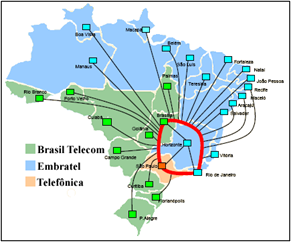
\includegraphics[width=.6\textwidth]{img/exemplo-conexoes.png}
    \legend{Fonte: \citeonline{rappaport09}}
\end{figure}

Se a figura que for incluída se tratar de um diagrama, um gráfico ou uma ilustração de autoria própria, priorize o uso de imagens vetoriais no formato PDF. Com isso, o tamanho do arquivo final do trabalho será menor, e as imagens terão uma apresentação melhor, principalmente quando impressas, uma vez que imagens vetoriais são perfeitamente escaláveis para qualquer dimensão. Veja o próprio logo do PPGEE, presente na capa e na folha de rosto, que está no formato PDF, bem como a \autoref{fig:exemplo-mlp}. Se for utilizar o Microsoft Excel para produzir gráficos, ou o Microsoft Word para produzir ilustrações, exporte-os como PDF e os incorpore ao documento.

\begin{figure}[htbp]
    \centering
    \caption{\label{fig:exemplo-mlp} Rede neural \textit{perceptron} de arquitetura 2-NH-1.}
    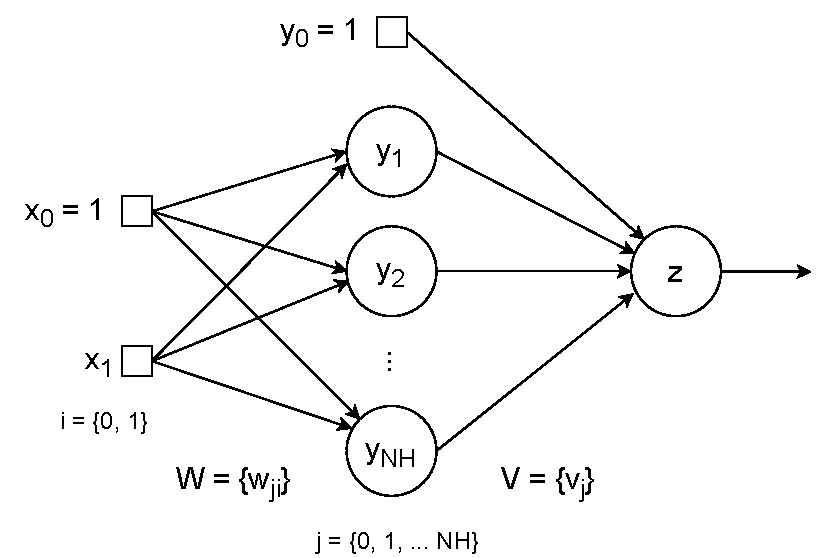
\includegraphics[width=.6\textwidth]{img/exemplo-mlp.pdf}
    \legend{Fonte: autoria própria.}
\end{figure}

Veja também a ferramenta Inkscape (\url{http://inkscape.org/}). Ela é uma excelente opção de código-livre para produzir ilustrações vetoriais, similar ao CorelDraw ou ao Adobe Illustrator. Para produzir diagramas, há também a ferramenta online \url{https://www.diagrams.net/}, que também permite a exportação direto para o formato PDF. O diagrama da \autoref{fig:exemplo-mlp} foi feito utilizando esta ferramenta.

De todo modo, caso não seja possível utilizar arquivos de imagens como PDF, pode-se utilizar qualquer outro formato, como JPEG (preferencialmente para fotos), PNG (preferencialmente para texto, diagramas ou desenhos simples) etc.

O \LaTeX{} também permite inserir subfiguras. Veja o exemplo da \autoref{fig:exemplo-subfiguras}. Pode-se também referenciar as subfiguras individualmente (\autoref{fig:subfig1} e \autoref{fig:subfig2}).

\begin{figure}[htbp]
    \centering
    \caption{\label{fig:exemplo-subfiguras} Exemplo de subfiguras.}
    \begin{subfigure}[b]{0.45\textwidth}  % tamanho da subfigura
        \centering
        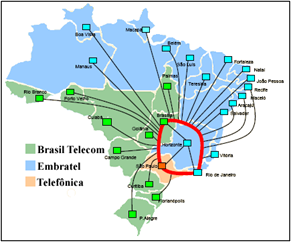
\includegraphics[width=\textwidth]{img/exemplo-conexoes.png}
        \caption{\label{fig:subfig1} subfigura à esquerda}
    \end{subfigure}
    \hfill
    \begin{subfigure}[b]{0.5\textwidth}  % tamanho da subfigura
        \centering
        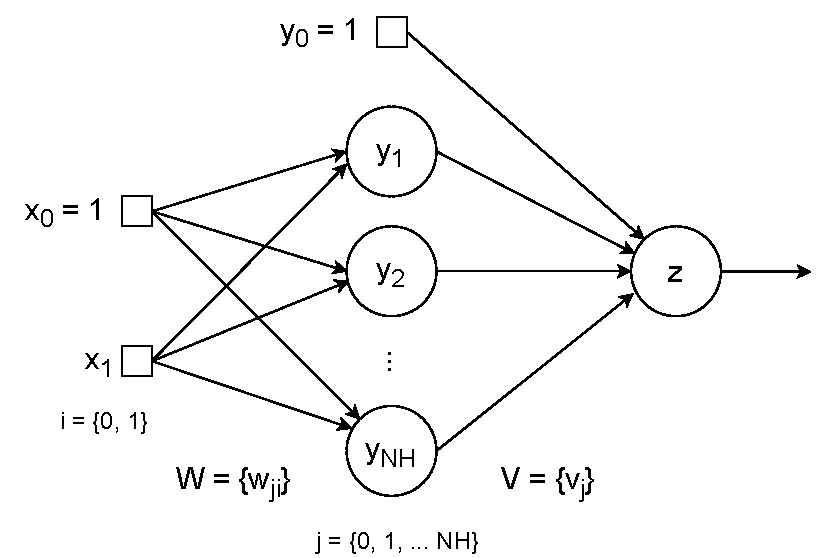
\includegraphics[width=\textwidth]{img/exemplo-mlp.pdf}
        \caption{\label{fig:subfig2} subfigura à direita}
    \end{subfigure}
\end{figure}

\subsection{Exemplo do Uso de Tabelas}

Em tabelas deve-se evitar o uso de bordas verticais para separar as colunas e bordas horizontais para separar as linhas. Somente o cabeçalho pode apresentar bordas horizontais para separar os títulos das colunas. Ao final da tabela é utilizada uma borda horizontal. Veja o exemplo da \autoref{tab:exemplo}.

\begin{table}[htb]
    \centering
    \caption{\label{tab:exemplo} Atividades desenvolvidas.}
    \begin{tabular}{ll}
        \toprule
        PERÍODO & ATIVIDADE \\
        \midrule
        EM 2006 (DEZ) & - Treinamento\\
        EM 2008 (JAN/FEV/MAR) & - Atividades de Gerenciamento de Redes\\
        & - Manutenção da Rede Física de Dados e Voz Local\\
        \bottomrule
    \end{tabular}
\end{table}

Pode-se utilizar a ferramenta online \url{https://www.tablesgenerator.com/} para elaborar tabelas \LaTeX{} de forma visual. Mude a opção ``\textit{Default table style}'' para ``\textit{Booktabs table style}'' (não precisa incluir o pacote \texttt{booktabs}, a classe \texttt{ppgee} já inclui este pacote).

\subsection{Exemplo do Uso de Alíneas}

Quando for necessário enumerar diversos assuntos de uma seção que não possua título, esta deve ser subdividida em alíneas. As alíneas, segundo a ABNT NBR 6024, devem ser apresentadas da seguinte forma:

\begin{alineas}
    \item Primeira Alínea:
    \begin{subalineas}
        \item Outros dados adicionais.
    \end{subalineas}
    
    \item Segunda Alínea:
    \begin{subalineas}
        \item Dados adicionais.
    \end{subalineas}
\end{alineas}


\subsection{Citação no Texto}

As citações devem ser indicadas no texto por um sistema de chamada: numérico ou autor-data \cite{NBR6023}. A seleção do sistema de chamada é feita no cabeçalho do arquivo \LaTeX, como opção do pacote \texttt{abntex2cite}. Para usar o sistema numérico, use a opção \verb|[num]|, ou para usar o sistema autor-data, use a opção \verb|[alf]|.

\begin{verbatim}
\usepackage[num]{abntex2cite}  % sistema numérico; ou
\usepackage[alf]{abntex2cite}  % sistema autor-data
\end{verbatim}

As citações podem ser diretas (somente no sistema autor-data): ``De acordo com \citeonline{engelbrecht2007}...''; ou indiretas \cite{engelbrecht2007}. Consulte o manual do pacote \texttt{abntex2cite} \cite{abntex2cite} para mais informações sobre o sistema numérico, ou o documento suplementar \texttt{abntex2cite-alf} \cite{abntex2cite-alf} para mais informações sobre o sistema autor-data.

A ABNT NBR 10520:2002, seção 5.3, descreve que citações diretas com mais de três linhas devem ser destacadas com recuo de 4 cm da margem esquerda, com letra menor que a do texto utilizado e sem as aspas. Para inserir citações longas, utilize o ambiente \texttt{citacao}, conforme o exemplo:

\begin{citacao}
As citações diretas, no texto, com mais de três linhas, devem ser destacadas com recuo de 4 cm da margem esquerda, com letra menor que a do texto utilizado e sem as aspas. No caso de documentos datilografados, deve-se observar apenas o recuo \cite[5.3]{NBR10520}
\end{citacao}

O ambiente \texttt{citacao\oarg{language}} pode receber como parâmetro opcional um nome de idioma previamente carregado nas opções da classe. Nesse caso, o texto da citação é automaticamente escrito em itálico e a hifenização é ajustada para o idioma selecionado na opção do ambiente, conforme o exemplo:

\begin{citacao}[english]
But what is intelligence? Dictionaries define intelligence as the ability to comprehend, to understand and profit from experience, to interpret intelligence, having the capacity for thought and reason (especially to a high degree). Other keywords that describe aspects of intelligence include creativity, skill, consciousness, emotion and intuition. \cite{engelbrecht2007}
\end{citacao}

